\documentclass[10pt,a4paper]{article}
\usepackage[margin=0.8in]{geometry}
\usepackage[T1]{fontenc}
\usepackage[utf8]{inputenc}
\usepackage{lmodern,amsmath,amssymb,booktabs,array,enumitem}
\usepackage[expansion=false]{microtype}
\usepackage{csquotes}
\usepackage{xurl,hyperref,tabularx,graphicx,xcolor}
\usepackage[section]{placeins}
\usepackage{longtable}
\setlength{\emergencystretch}{2em}
\hypersetup{hidelinks}
\newcolumntype{Y}{>{\raggedright\arraybackslash}X}
\newcolumntype{L}[1]{>{\raggedright\arraybackslash}p{#1}}
\setlength{\parindent}{0pt}
\setlength{\parskip}{4pt}
\setlength{\tabcolsep}{3pt}
\renewcommand{\arraystretch}{1.12}
\setlist{nosep,leftmargin=*}
\newcommand{\figw}{\linewidth}

\title{\textbf{Computer Networks --- Research Project}\\[4pt]
\large Phase 3: Implementation, Experiments and Results\\[8pt]
\Large Poisoning, Retention and Legitimate Adaptation\\in Federated Continual Intrusion Detection}
\author{Saneedullah (23I-2568) \qquad Ahmed Bilal (23I-2581)}
\date{Audited revision: 16 November 2026}


\begin{document}
\maketitle
\begin{abstract}
We audit and revise a five-client, four-stage federated continual intrusion-detection study against its original Phase 2 commitments. The original submitted report and stronger majority-attacker experiments are preserved as historical exploratory artifacts. Independently verified newer evidence contains 240 primary single-attacker trajectories across twelve ownership seeds, 168 additional control/ablation trajectories, nine clean confirmations, and 24 oracle continuations. All outcomes use a reused development bank, not an independent final test. Source and input checks, exact count-based endpoints, paired controls and checkpoint hashes support conditional reproducibility. In the clean primary comparison, class-aware admission DC has acquisition 0.296 versus matched-global DM 0.399, and benign false-alarm fractions 0.114 versus 0.056. Replay's immediate single-attacker Hulk recall change is small at the maximum prescribed dose; this limits broad persistence claims. Original significance claims are withdrawn because training repetitions share only three ownership partitions and the submitted multiplicity/endpoint definitions differ from Phase 2. The revised conclusions retain adverse findings, distinguish mechanism evidence from causal speculation, and identify unresolved raw-session reconstruction, external evaluation and sealed-test qualification.
\end{abstract}
\section{Introduction and Scope}
The scientific questions from the submitted report are retained:
\begin{itemize}
\item \textbf{RQ1:} How do fine-tuning, an EWC-style regulariser and DER++ replay differ in immediate source-family damage and later error after attacker withdrawal?
\item \textbf{RQ2:} How does class-aware admission change poisoning damage, legitimate acquisition and false alarms relative to a volume-matched global filter?
\item \textbf{RQ3:} What do matched interventions and component ablations establish about memory/selection mechanisms and computational costs?
\end{itemize}
This revision uses the actual pre-deadline report TeX as its editorial foundation: its research questions, implementation/data/evaluation structure and source class table are retained. Historical numerical results and claims are not silently relabelled as new evidence. The original report PDF/TeX and ZIP remain unchanged. The complete issue register and commitment-to-evidence matrix accompany this report.

\subsection{What changed from the Phase 2 plan}
The corrected release uses 74 inputs after omitting forward/backward header-length fields, sixteen annotated labels, and widths 3/8/13/16. E3 acquisition is supported principally by the annotated Infiltration--Portscan scenario; its distinction from Friday PortScan does not certify a distinct new technique. Data/taxonomy adoption records are separate from instructor feedback, which was not supplied.

The original submission's stronger 3/5-attacker study was an exploratory escalation. Calling it a predeclared fallback was inaccurate: Phase 2 explicitly states that a weak effect must not trigger extra attackers or higher doses. Historical experiments use three ownership partitions with four training repetitions each. These are not twelve independent ownership partitions. The newer primary comparison instead uses seeds 1--11 and 42, one attacker, doses 0/.1/.3/.5 and an unchanged threat. Development reuse still prevents confirmatory final-test interpretation.

\section{Implementation of the Proposed Methodology}
\subsection{Federation and model}
The audited newer engine simulates five persistent clients with whole-component Dirichlet(.5) ownership. Each stage has twelve rounds and one local epoch. An MLP maps 74 inputs through 128/64 ReLU layers with dropout .1 to a trainable expanding head. Appended head blocks use Xavier-uniform weights and zero bias, retaining old rows. The class registry uses supplied current labels. Adam resets on broadcasts; active clients are weighted by distinct admitted current rows, excluding replay and repeated epochs. The current learning implementation is frozen separately from orchestration corrections.

\subsection{Learners and admission rules}
FT uses current cross-entropy. EI accumulates client-local per-example squared-gradient empirical Fisher, sampled without replacement up to 1,024 admitted current rows, with dropout off and a final-aggregate anchor. Importance is not averaged across clients. This differs materially from the historical engine's global averaged importance; the historical EI is not an implementation of the proposed local-EI baseline.

DR uses 500 replay slots per client, first-pass-only Algorithm R insertion, 128-record replay draws without replacement, pre-update evaluation-mode teachers, separate draw/insertion streams, and observed-width-normalized logit matching. Current/replay cross-entropy uses training-mode dropout; logit matching retains gradients with dropout off. DC protects supplied new classes and classes with fewer than twenty local records; remaining supplied classes receive a ceiling-rounded quota. DM ranks globally but admits the same per-client total. In this schedule benign is the recurring current class: protection does not establish generic balancing of recurrent attack classes. DQ uses the same class quotas with random within-class ranking. Phase 2's separate DG baseline, DER++ with a fixed global 75\% low-loss filter, now has a deterministic selector implementation but no adopted-profile outcome runs. DG is not DM's volume-matched global ranking and is not DQ's random-within-quota rule; therefore the current matrix is not a complete Phase 2 baseline comparison.

One uniformly eligible client corrupts nested random prefixes of its E2 Hulk labels to benign. Features are unchanged. E3/E4 introduce no fresh Hulk or corruption. Oracle continuations clone E2 state and repair only stored poisoned labels; earlier weights and teachers remain poisoned. These are explanatory interventions, not deployable defences.

\subsection{Engineering and reproducibility}
The starting checkout is commit \texttt{a2e2fe3b67db9cd3b180ecfa59c4c898a94a73c0} plus preserved uncommitted work. Both original ZIP copies hash to the same value. The recorded overnight runner was recovered byte-for-byte; the pre-audit current runner differed only in scheduling reserve. A later audit patch scopes an admission adapter that previously mutated the shared v2 chooser on import. Frozen source is preserved, rather than rewriting its identity.

Across the two newer result trees, 963 physical result files collapse to 417 unique configurations; 546 are identical copies. There are no conflicting duplicate payloads. All recorded source dependencies except the disclosed runner drift, all 26 pinned input files, all completion payload hashes and all 1,668 saved stage-weight hashes pass their checks. Run counts separate ownership seeds, complete trajectories and 24 embedded E3/E4 oracle branches. Repeated E1 weights establish pairing, not evidence that every historical job physically reused computation.

\section{Dataset and Preprocessing}
The corrected CICIDS2017 source is a revised extraction/annotation of the same historical capture, not an independent dataset \cite{liu}. Ports, addresses, timestamps and labels are not predictors. Monday-only T0 has 371,621 fitting rows. The frozen min--max transform is not clipped or refitted; zero ranges use denominator one. There are 183,045 selected training and 272,506 development rows. Every exported input was independently reconstructed from T0 with zero mismatched FP32 cells.

Recorded train/development/test component assignments have zero cross-role overlap, zero T0-closure or excluded records in assigned inventory, and no exported role errors. Training/development IDs and transformed feature content have zero overlap; fresh stage IDs are disjoint. An independent full-SHA256/sparse-connectivity reconstruction reparsed source metadata and exactly recovered the120s graph and T0 closure. At60s the frozen split remains component-disjoint;300s grouping instead joins8,982 train/development components (and9,056 train/test,3,444 development/test). Isolation is conditional on the declared120s grouping. Source CSV-to-metadata parsing is still an upstream dependency; operational grouping does not certify true application sessions. No final-test feature or label payload was opened.
\begin{table}[htbp]
\centering\footnotesize
\caption{Classes of the corrected CICIDS2017 benchmark: arrival stage, scoring eligibility and rows (training package of seed 101; fixed development bank).}
\label{tab:classes}
\begin{tabularx}{\linewidth}{rYcccr}
\toprule
Code & Class & Arrives & Scored & Train rows & Dev rows\\
\midrule
0 & Benign & E1 & yes & 14,000 & 216,158\\
1 & Bot & E4 & yes & 441 & 148\\
2 & DDoS & E4 & yes & 57,086 & 19,029\\
3 & DoS GoldenEye & E2 & yes & 4,540 & 1,513\\
4 & DoS Hulk & E2 & yes & 95,080 & 31,694\\
5 & DoS Slowhttptest & E2 & yes & 1,037 & 346\\
6 & DoS Slowloris & E2 & yes & 2,071 & 691\\
7 & FTP-Patator & E1 & yes & 2,382 & 795\\
8 & Heartbleed & E2 & no & 11 & 0\\
9 & Infiltration & E3 & no & 27 & 5\\
10 & Infiltration - Portscan & E3 & yes & 3,591 & 1,198\\
11 & PortScan & E4 & yes & 943 & 315\\
12 & SSH-Patator & E1 & yes & 1,776 & 592\\
13 & Web Attack Brute Force & E3 & no & 43 & 15\\
14 & Web Attack Sql Injection & E3 & no & 7 & 3\\
15 & Web Attack XSS & E3 & no & 10 & 4\\
\bottomrule
\end{tabularx}
\end{table}
\section{Experimental Setup and Baseline Evaluation}
The primary matrix is five methods (FT/EI/DR/DM/DC), four doses and twelve ownership seeds: 240 full trajectories. Additional completed blocks are DQ clean/.5 (24), two DC loss removals clean/.5 (48), and DM/DC alternative quotas .50/.90 clean/.5 (96). The nine pilot confirmations are development seeds 101--103. Oracle continuations number 24, DR and DC at dose .5. Do not pool this evidence with the original 696 GPU configurations or the earlier CPU supplements as if they add independent ownership seeds.

The original mean clean gates pass, but FTP acquisition is zero for pilot seed103 for each learner while the three-seed mean is .667. The gate does not promise every partition learns the anchors. No seed is discarded and no gate is changed after observing outcomes.

Eligible macro-F1 restricts true rows to the fixed eligible seen set and retains every predicted column. Descriptive full-inventory performance includes supported rare families; Heartbleed has no development support and cannot receive a held-out score. Precision is undefined for an unpredicted class, whereas supported recall/F1 are zero. Averages never silently drop fixed eligible classes.
\begin{center}\small
\begin{tabular}{llll}
\toprule
Method & Eligible F1 & Acquisition A & Benign FAR\\
\midrule
FT & 0.106 & 0.252 & 0.442\\
EI & 0.111 & 0.214 & 0.363\\
DR & 0.627 & 0.390 & 0.063\\
DM & 0.589 & 0.399 & 0.056\\
DC & 0.505 & 0.296 & 0.114\\
\bottomrule
\end{tabular}
\end{center}
\begin{center}\small
\begin{tabular}{llll}
\toprule
Method & Fixed-cohort ACC & BWT & Forgetting\\
\midrule
FT & 0.527 & -0.484 & 0.488\\
EI & 0.592 & -0.405 & 0.408\\
DR & 0.943 & -0.032 & 0.037\\
DM & 0.948 & -0.006 & 0.034\\
DC & 0.902 & -0.037 & 0.051\\
\bottomrule
\end{tabular}
\end{center}
These clean metrics are recomputed from 240 checkpoints (60 trajectories); their regenerated stage confusion matrices match exactly. ACC equally weights fixed stage cohorts, each with its disjoint benign component cohort. It is not pooled accuracy. Historical reported BWT/forgetting instead average attack-family recalls and are not substituted here. Low pooled or cohort error can coexist with poor minority-family macro-F1.

\section{Poisoning and Defences}
Define $H=\frac12\sum_{t=3}^4(ASR_t^\rho-ASR_t^0)$ using the fixed Hulk bank, where ASR is Hulk predicted benign. Immediate damage is signed poisoned-minus-clean E2 Hulk recall. Acquisition $A$ equally averages E2--E4 means over eligible newly introduced untargeted families. Clean E4 FAR uses the same 216,158 benign records. These estimands distinguish source damage, forgetting and acquisition; H is not final recall loss.
\begin{center}\small
\begin{tabular}{lllll}
\toprule
Method & $\Delta$rec (.5) & H (.5) & A (.5) & FAR (.5)\\
\midrule
FT & -0.0001 & +0.1397 & +0.2711 & +0.4707\\
EI & -0.0002 & +0.0882 & +0.2161 & +0.3920\\
DR & -0.0006 & +0.0087 & +0.3883 & +0.0604\\
DM & -0.0168 & +0.0112 & +0.3845 & +0.0560\\
DC & -0.0001 & +0.0003 & +0.2867 & +0.1311\\
\bottomrule
\end{tabular}
\end{center}
\begin{figure}[!htbp]
\centering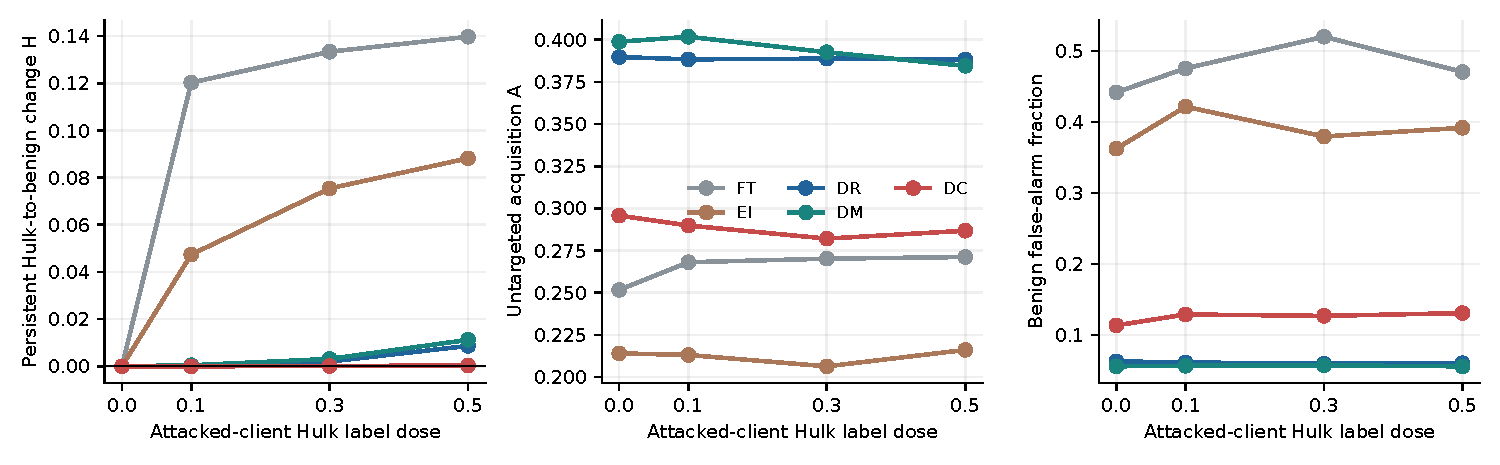
\includegraphics[width=\linewidth]{figures/primary-tradeoffs.pdf}
\caption{Means over twelve ownership-seeded development trajectories. Dose is the attacked client's Hulk fraction, not a fixed global corruption rate. H already subtracts the paired clean run; A and FAR are absolute fractions. Lines summarize seeds and do not show cross-capture uncertainty.}
\end{figure}
Clean DC minus DM acquisition is -0.1030 (descriptive 95\% whole-seed interval [-0.1285, -0.0758]); clean FAR is +0.0576, or about 576 additional false alerts per 10,000 benchmark benign flows. The latter is not a daily production forecast.
DC has lower mean acquisition at every tested dose and higher clean false alarms. Retaining all supplied new-class rows does not establish better learning. Conversely, a small H with poor clean retention is not evidence of a secure model: show absolute clean and poisoned performance alongside the difference. Replay's maximum-dose immediate recall change is approximately -0.00064. A strong general attack-persistence claim is therefore not supported by the prescribed single-attacker immediate effect.
\begin{figure}[!htbp]
\centering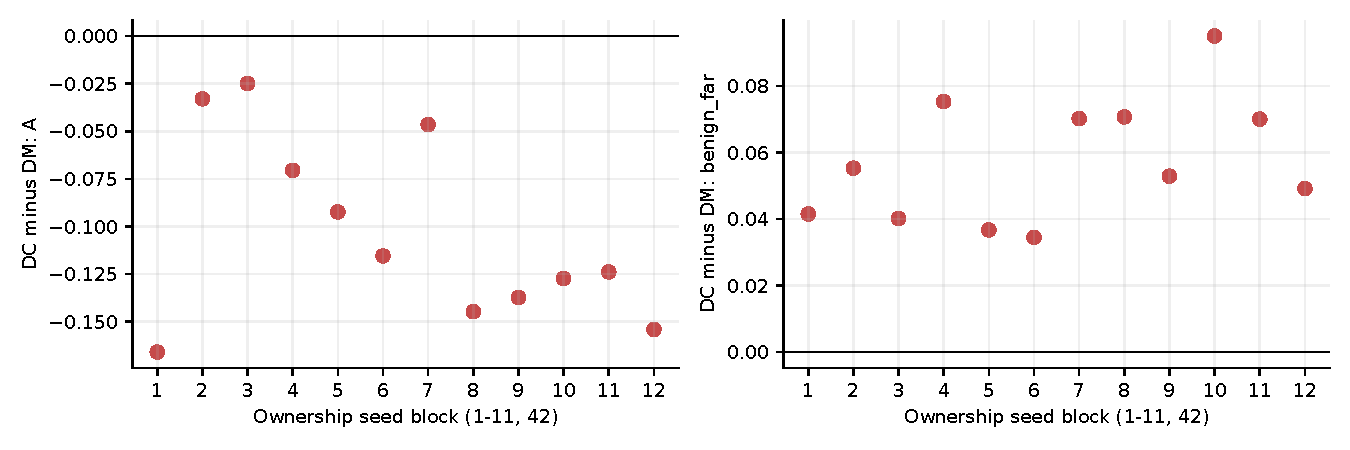
\includegraphics[width=\linewidth]{figures/paired-effects.pdf}
\caption{Clean paired DC-minus-DM effects for all twelve ownership blocks. Points are training/ownership variability on one fixed capture and split; no independent-site uncertainty is implied.}
\end{figure}
\subsection{Admission and retained-poison diagnostics}
The saved ledgers show identical per-client, per-supplied-class raw counts and quotas for DM and DC at every stage and dose (192 paired stage comparisons). The selected ID sets still differ: 109/240 client-stage pairs at dose .5 have different per-client admitted-set hashes. Thus quota counts alone do not explain the outcome contrast; the hashes do not reveal which examples or loss ranks changed. At dose .5, known poisoned IDs in the five replay buffers average 163.1 under DM versus 131.0 under DC at E2 (paired DC-DM -32.1, bootstrap 95\% interval [-45.4, -19.1]) and 117.0 versus 92.1 at E4. The lower stored-poison count under DC is consistent with different selected examples, but memory occupancy is not replay draw or gradient exposure. The family F1 panel shows heterogeneous E4 changes under the reused development bank; it does not isolate the contribution of scores, exposure, or aggregation weights. Per-example score vectors, replay draws, and per-client aggregation weights were not retained, so the cause of DC's higher benign FAR and lower acquisition remains unidentified.
\begin{figure}[!htbp]
\centering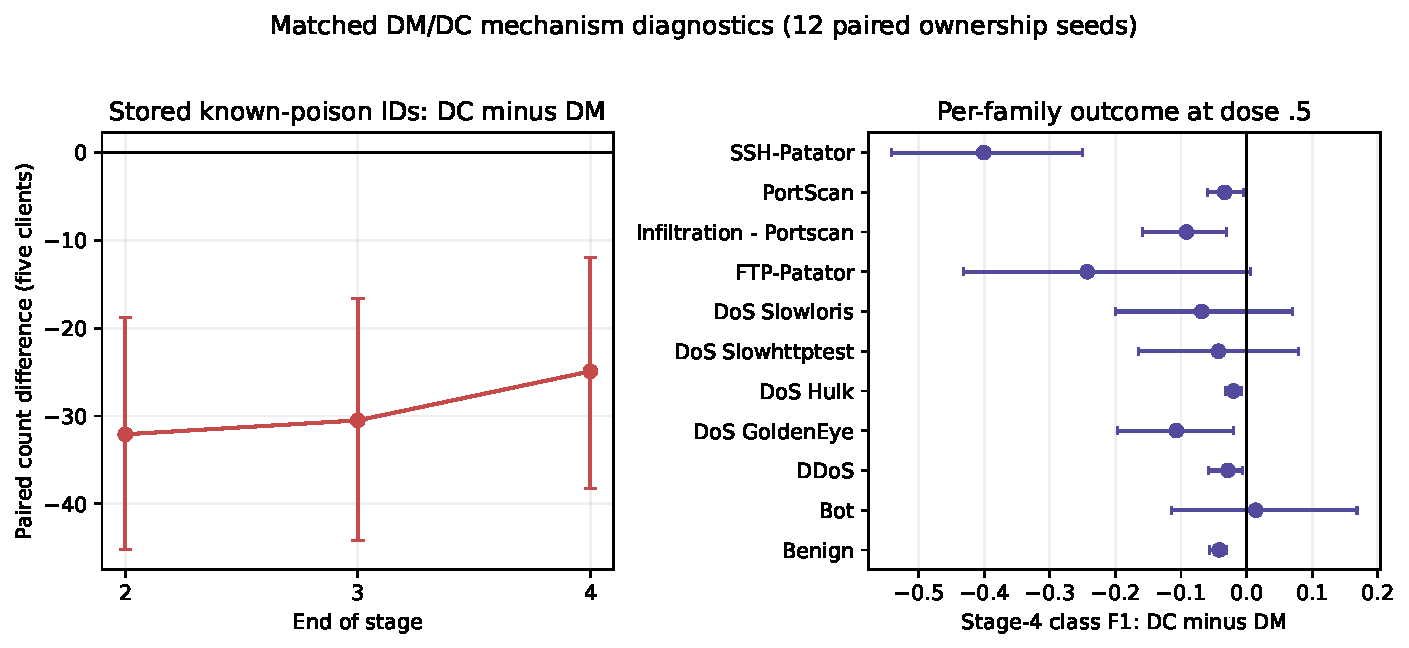
\includegraphics[width=\linewidth]{figures/admission-mechanism-diagnostic.pdf}
\caption{Matched primary DR DM/DC runs on the reused development bank (12 ownership seeds). Left: DC-minus-DM difference in known poisoned IDs stored across five 500-slot buffers at ends of stages 2--4; points and 95\% intervals bootstrap whole paired ownership seeds. Right: stage-4 per-family F1 DC-minus-DM at dose .5 for eligible classes; 95\% intervals resample whole ownership seeds. Paired per-client class quotas are identical while admitted-set hashes differ for 109/240 client-stage pairs. Descriptive only; stored occupancy is not replay exposure.}
\end{figure}
\subsection{Inference and sensitivity}
All 29 original contrast slots are retained in one Holm family. C1 uses learner pairs on H and immediate recall change (18); C2 uses acquisition (4), H/recall change (6), and clean FAR (1). Count-derived rational differences give exact ties/zeros, averaged ranks, and conditional sign enumeration. H/recall differences subtract clean exactly once. All-zero contrasts have p=1 and rank-biserial effect zero. Descriptive percentile intervals resample whole paired ownership seeds 10,000 times and are not simultaneous intervals.

Five signed-rank contrasts survive Holm: DC-minus-DM acquisition at doses0/.1/.3, clean FAR, and the remaining contrast identified in the complete table. Exact enumeration does not remove the symmetry assumption. The sign-test sensitivity is reported for every contrast; at dose .1 acquisition it does not survive its separate exploratory sensitivity correction. Treat divergence as a limitation, not a choice between favorable tests. The fixed reused development bank means neither family is a new confirmatory final-test result. Non-significance does not establish equivalence.
\begin{longtable}{llllrrr}
\toprule
Pair & Endpoint & Dose & Mean diff. & Holm p & Sign p* & Nonzero\\
\midrule
\endhead
FT-EI & H & 0.1 & +0.0729 & 1.0000 & 1.0000 & 12\\
FT-EI & H & 0.3 & +0.0580 & 1.0000 & 1.0000 & 12\\
FT-EI & H & 0.5 & +0.0515 & 0.7178 & 0.8486 & 12\\
FT-DR & H & 0.1 & +0.1200 & 0.0254 & 0.0254 & 11\\
FT-DR & H & 0.3 & +0.1314 & 0.7178 & 1.0000 & 12\\
FT-DR & H & 0.5 & +0.1311 & 0.2808 & 0.1587 & 12\\
EI-DR & H & 0.1 & +0.0471 & 1.0000 & 1.0000 & 12\\
EI-DR & H & 0.3 & +0.0734 & 1.0000 & 1.0000 & 12\\
EI-DR & H & 0.5 & +0.0795 & 1.0000 & 1.0000 & 12\\
FT-EI & delta\_recall & 0.1 & +0.0000 & 1.0000 & 1.0000 & 6\\
FT-EI & delta\_recall & 0.3 & +0.0002 & 1.0000 & 1.0000 & 6\\
FT-EI & delta\_recall & 0.5 & +0.0002 & 1.0000 & 1.0000 & 8\\
FT-DR & delta\_recall & 0.1 & +0.0000 & 1.0000 & 1.0000 & 9\\
FT-DR & delta\_recall & 0.3 & +0.0000 & 1.0000 & 1.0000 & 7\\
FT-DR & delta\_recall & 0.5 & +0.0006 & 1.0000 & 1.0000 & 8\\
EI-DR & delta\_recall & 0.1 & +0.0000 & 1.0000 & 1.0000 & 7\\
EI-DR & delta\_recall & 0.3 & -0.0002 & 1.0000 & 1.0000 & 7\\
EI-DR & delta\_recall & 0.5 & +0.0004 & 1.0000 & 1.0000 & 9\\
DC-DM & A & 0.0 & -0.1030 & 0.0142 & 0.0142 & 12\\
DC-DM & A & 0.1 & -0.1119 & 0.0366 & 0.1587 & 12\\
DC-DM & A & 0.3 & -0.1105 & 0.0142 & 0.0142 & 12\\
DC-DM & A & 0.5 & -0.0977 & 0.1641 & 0.1587 & 12\\
DC-DM & H & 0.1 & -0.0005 & 1.0000 & 1.0000 & 9\\
DC-DM & H & 0.3 & -0.0030 & 0.4297 & 1.0000 & 10\\
DC-DM & H & 0.5 & -0.0109 & 0.7979 & 1.0000 & 11\\
DC-DM & delta\_recall & 0.1 & +0.0005 & 1.0000 & 1.0000 & 8\\
DC-DM & delta\_recall & 0.3 & +0.0046 & 1.0000 & 1.0000 & 10\\
DC-DM & delta\_recall & 0.5 & +0.0167 & 1.0000 & 1.0000 & 11\\
DC-DM & benign\_far & 0.0 & +0.0576 & 0.0142 & 0.0142 & 12\\
\bottomrule\end{longtable}
* Separate exploratory Holm correction of 29 sign-test sensitivities; not an additional confirmatory family.
\section{Ablation Studies and Mechanism Limits}
The latest loss ablations remove the logit or replay-label term on DC, with configuration-specific clean twins. Quota changes are matched for DM and DC at .50/.75/.90. Completed blocks are incorporated here rather than left only in an addendum. All contrasts are exploratory and are not retuned.
\begin{center}\small
\begin{tabular}{llll}
\toprule
Variant (.5 dose) & H & A & FAR\\
\midrule
DQ random quotas & 0.0008 & 0.3469 & 0.0780\\
DC no logits & 0.0026 & 0.2744 & 0.1852\\
DC no replay labels & 0.0454 & 0.1361 & 0.4679\\
\bottomrule
\end{tabular}
\end{center}
\begin{figure}[!htbp]
\centering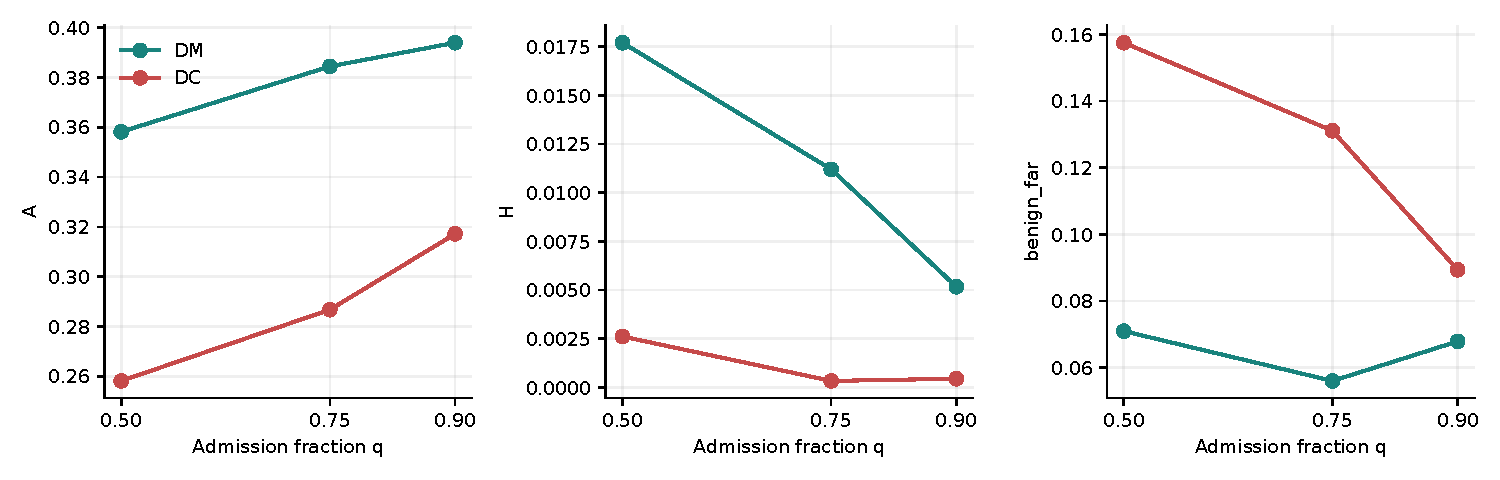
\includegraphics[width=\linewidth]{figures/quota-ablations.pdf}
\caption{Matched quota ablation means over twelve ownership seeds at dose .5. The .75 reference is reused from the primary study, not counted as newly executed trajectories. Changed settings use their own clean twins for H.}
\end{figure}
Oracle repair changes only labels of surviving poisoned IDs after E2, retaining weights, features, IDs, teacher logits, occupancy and random state. All 24 pairs are retained; there happen to be no zero-survivor cases in these data. Label repair does not reverse earlier weight/logit damage and estimates the downstream effect of this intervention, including later admission changes. Memory survival alone does not identify all persistence as caused by erroneous-label replay.
\begin{figure}[!htbp]
\centering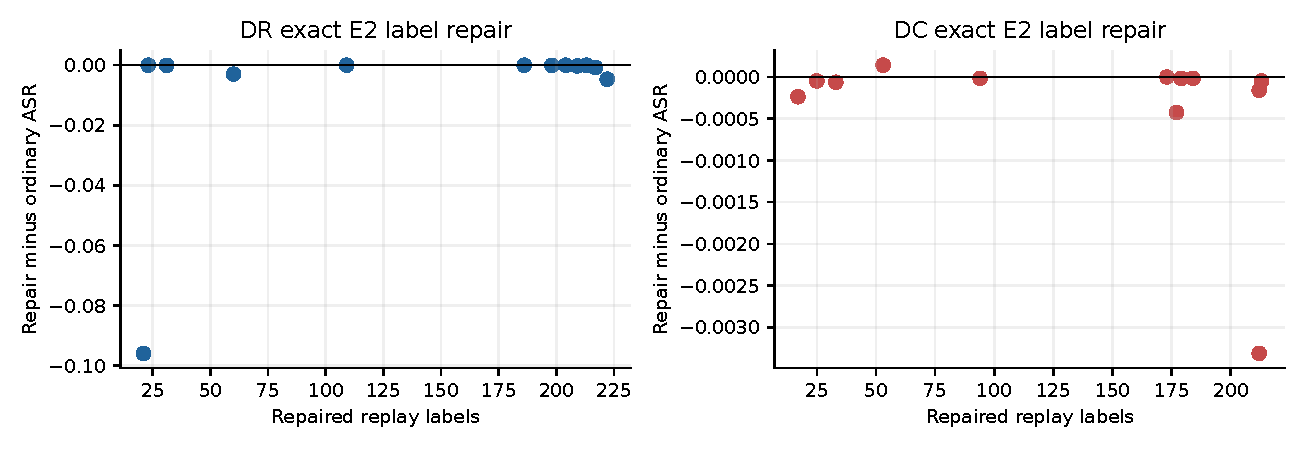
\includegraphics[width=\linewidth]{figures/oracle-repair.pdf}
\caption{Oracle repair minus ordinary continuation in mean E3/E4 Hulk-to-benign error. Each point is one seed; negative is lower error after repair. Repair counts are surviving memory labels, not newly supplied training records.}
\end{figure}
FIFO and the specifically prescribed class-balanced eviction are not validated in the latest single-attacker matrix. Historical FIFO outcomes from a different engine and stronger attack do not fill that gap. Accordingly, this report makes no claim that eviction explains the latest effect. An exact matched experiment card is supplied; omission narrows the mechanism conclusion rather than invalidating primary comparisons.

\subsection{RQ3: costs}
Stored whole-run elapsed times are not pure training cost: they include admission/evaluation and, in selected poisoned DR/DC runs, an oracle suffix. Their direct ratios are not fair method overhead comparisons. Existing pilot latency records use evaluation mode, batch1/256, ten warmups and100 trials; these are batch timings, not packet-processing or deployment throughput. A diagnostic replay (one seed each for FT, EI and DR/DC) recorded training, admission, importance (EI only) and evaluation categories; its three trajectories took 735.24 seconds total (results/phase3-rigorous-audit-v1/reproduction-attempt2/verification.json). This does not estimate method-level cost or variability. Figure~\ref{fig:observed-run-time} shows the distribution of per-trajectory elapsed wall time across all 417 unique adopted-profile results, after verifying completion-manifest hashes and collapsing 273 exact copies. Two quota-block DM trajectories at dose .5 and q=.5 took about 7,800 seconds each; these observations remain included and are not attributed to method overhead because component timings are unavailable. The full 408-run follow-up block took 32,655.01 seconds (9.07 hours) end to end, exceeding the planned six-hour CPU budget; elapsed time includes orchestration. No further training was scheduled. Historical communication estimates count raw model payloads, not measured serialization or label-registry traffic. Resource claims remain scoped to local simulation; no privacy, edge energy or network-latency guarantee is established.

\begin{figure}[!htbp]
\centering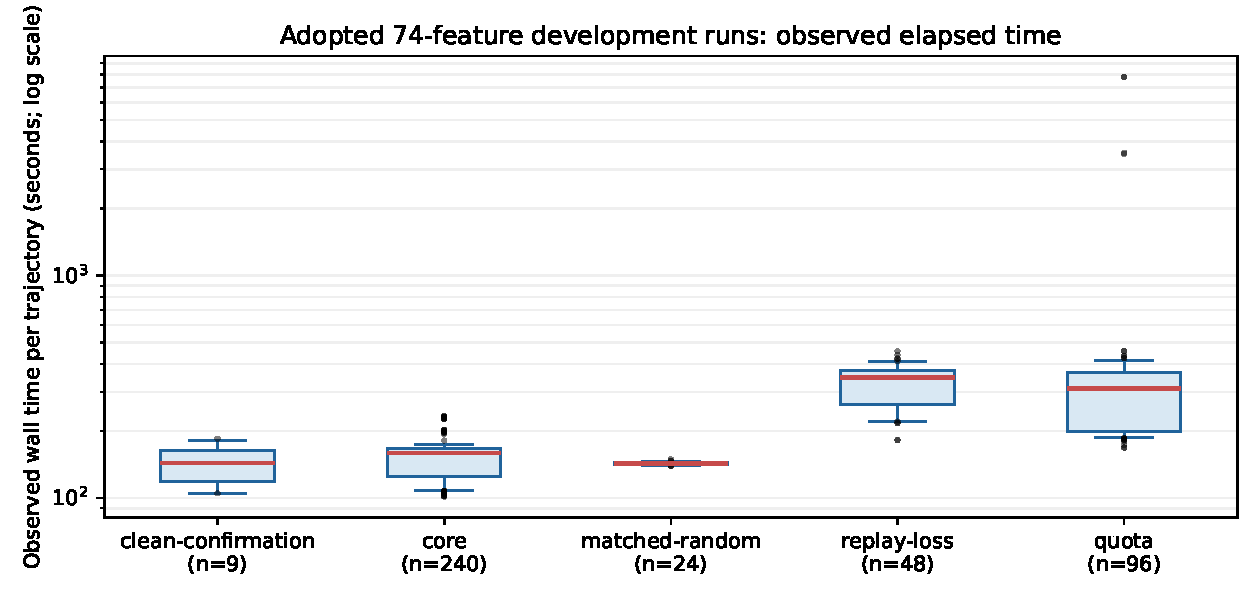
\includegraphics[width=0.94\linewidth]{figures/observed-run-time.pdf}
\caption{Observed runner wall time for unique adopted-profile trajectories by experimental block. Boxes show the interquartile range and median; whiskers use the 10th/90th percentiles; dots show outliers. The logarithmic scale preserves visibility of unusually long jobs. Values include orchestration and evaluation and are not training-only timings. Source table: \texttt{observed-run-costs.csv}.}
\label{fig:observed-run-time}
\end{figure}

\section{Comparison with Existing Research}
The primary author record for Lavaur et al. \cite{lavaur} supports dataset/hyperparameter-dependent label-flipping effects in a fixed-class federated IDS. It is context, not an accuracy baseline on our split. DER++ \cite{der} supplies the replay objective; observed-width normalization and expanding-head caching are declared adaptations. The corrected dataset authors \cite{liu} document why release, extraction and labeling provenance matter. Our corrected and original CICIDS2017 releases are the same underlying capture, so agreement between them is not independent external replication.

Recent related work by Wu et al. \cite{edgefedcil} studies federated class-incremental IDS with bounded replay and communication compression for edge IoT. Its data, architecture, participation protocol and communication measurements differ from this study, so it informs the design context only; its reported communication reduction is not a local baseline or directly comparable result.

We retain no numerical superiority ranking against incompatible published datasets, tasks or support populations. The source ledger records primary URLs and retained-PDF numerical checks. Broader literature numbers from the original submission are not reasserted as verified new findings. No universal novelty claim follows from the selected literature corpus.

\section{Analysis, Limitations and Conclusion}
The newer single-attacker evidence supports a reproducible conditional comparison of local-EI, replay and admission behavior on one reused development capture. Replay retains useful classification performance relative to unregularized/importance-only baselines, while DC does not establish a beneficial acquisition--false-alarm trade-off against DM. The immediate single-attacker replay effect is small. Strong historical majority-attacker damage cannot substitute for a result under the originally prescribed threat.

Reliability is strongest for verified raw counts, paired identities and regenerated development metrics. The original report's confirmatory statistics, predeclared-fallback characterization and exact Phase2-faithfulness claims must not be relied upon. Raw session-graph reconstruction, independent held-out evaluation, latest eviction controls, full cost characterization and external full-method validation remain incomplete. These are explicitly separated from confirmed implementation defects.

The external adapter pilot contains sixteen train-only arms on two datasets and one seed; it demonstrates execution only. Discovery-submodule outcomes are distinct exploratory evidence. Neither establishes external full-method effectiveness. No final-test payload was exported or scored in this audit. A role-enforced separate evaluator, verified isolation, frozen methods/checkpoints/analysis and a one-shot evaluation protocol are prerequisites; no outcome-driven tuning may follow.

Null and adverse findings remain valid. The contribution is correcting estimands, implementation boundaries and claims while retaining adverse results.

\section*{Availability and Requirement Map}
The package contains the audit register, traceability/checklists, experiment cards, patches/checks, unique results, recomputed metrics, report/figures and reproduction instructions. Rubric categories remain implementation(10), evaluation/comparison(10), ablation/validation(10); no score is promised. Original submission and historical source remain separate.

\begingroup\footnotesize
\begin{thebibliography}{9}\setlength{\itemsep}{0pt}
\bibitem{lavaur} L. Lavaur, Y. Busnel and F. Autrel. Investigating the Impact of Label-flipping Attacks against Federated Learning for Collaborative Intrusion Detection. \textit{Computers \& Security}, 156, 104462 (2025). DOI: \url{https://doi.org/10.1016/j.cose.2025.104462}.
\bibitem{der} P. Buzzega et al. Dark Experience for General Continual Learning: a Strong, Simple Baseline. NeurIPS2020. \url{https://arxiv.org/abs/2004.07211}.
\bibitem{liu} L. Liu et al. Error Prevalence in NIDS datasets: A Case Study on CIC-IDS-2017 and CSE-CIC-IDS-2018. IEEE CNS2022,254--262. \url{https://intrusion-detection.distrinet-research.be/CNS2022/index.html}.
\bibitem{edgefedcil} Z. Wu et al. Communication-Efficient Federated Class-Incremental Intrusion Detection for Edge IoT Networks. \textit{Sensors}, 26(14), 4630 (2026). DOI: \url{https://doi.org/10.3390/s26144630}.
\end{thebibliography}
\endgroup

\end{document}
